% ===================================================================
\chapter{Evaluation Method}
\label{ch:evaluation}

\section{Two stages}
\label{sec:stages}

The evaluation runs in two stages, each answering one question.

\paragraph{Stage 1 --- which methods are worth building?}
All eight methods of Section~\ref{sec:candidates} are run in MATLAB over the
same 50 consecutive ColoRadar frames with all 16 receive channels. Each is
scored on compression ratio and on what it does to target detection. A method
goes forward only if it is lossless --- it loses no detections beyond those of
the FX16 step every method shares --- and compresses by more than three, which
leaves a margin over the \num{2.4}--\num{2.7} that a Gigabit Ethernet link needs
(Section~\ref{sec:kiem} and Chapter~\ref{ch:kiem}).

\paragraph{Stage 2 --- where does the compression come from, and what does it
cost in hardware?}
The selected methods, DRHE and LPC, are evaluated on the four-receiver frames
that the hardware processes. Their compression ratio is broken down into what
the entropy coder achieves alone, what prediction adds, and what a re-derived
dictionary adds. They are then implemented, with decoders, in hardware
(Chapter~\ref{ch:hardware}), verified bit for bit at every level of the ladder
of Section~\ref{sec:ladder}, and measured on the board for time per frame,
latency and chip resources.

\section{The reference signal chain}
\label{sec:refchain}

A ColoRadar frame is read and reshaped into a complex cube of (fast time
$\times$ ramp $\times$ receiver) with the TDM flattening of
Equation~\eqref{eq:rampindex}, and the per-ramp mean is subtracted to remove
the DC and transmitter-leakage term. A Hann window is applied along fast time,
and an $N_s$-point range FFT normalised by $N_s$. Only the positive half of the
spectrum is kept, giving 128 range bins; the input is complex, so this is a
choice to keep positive ranges, not a consequence of symmetry. The result is
scaled by Equation~\eqref{eq:scale} and rounded to \texttt{int16}. Four
receive channels are exported to the hardware path, because four complex
\texttt{int16} samples make one 128-bit AXI4-Stream beat; one such frame is
\SI{393216}{\byte} (Figure~\ref{fig:input}).

\begin{figure}[htbp]
\centering
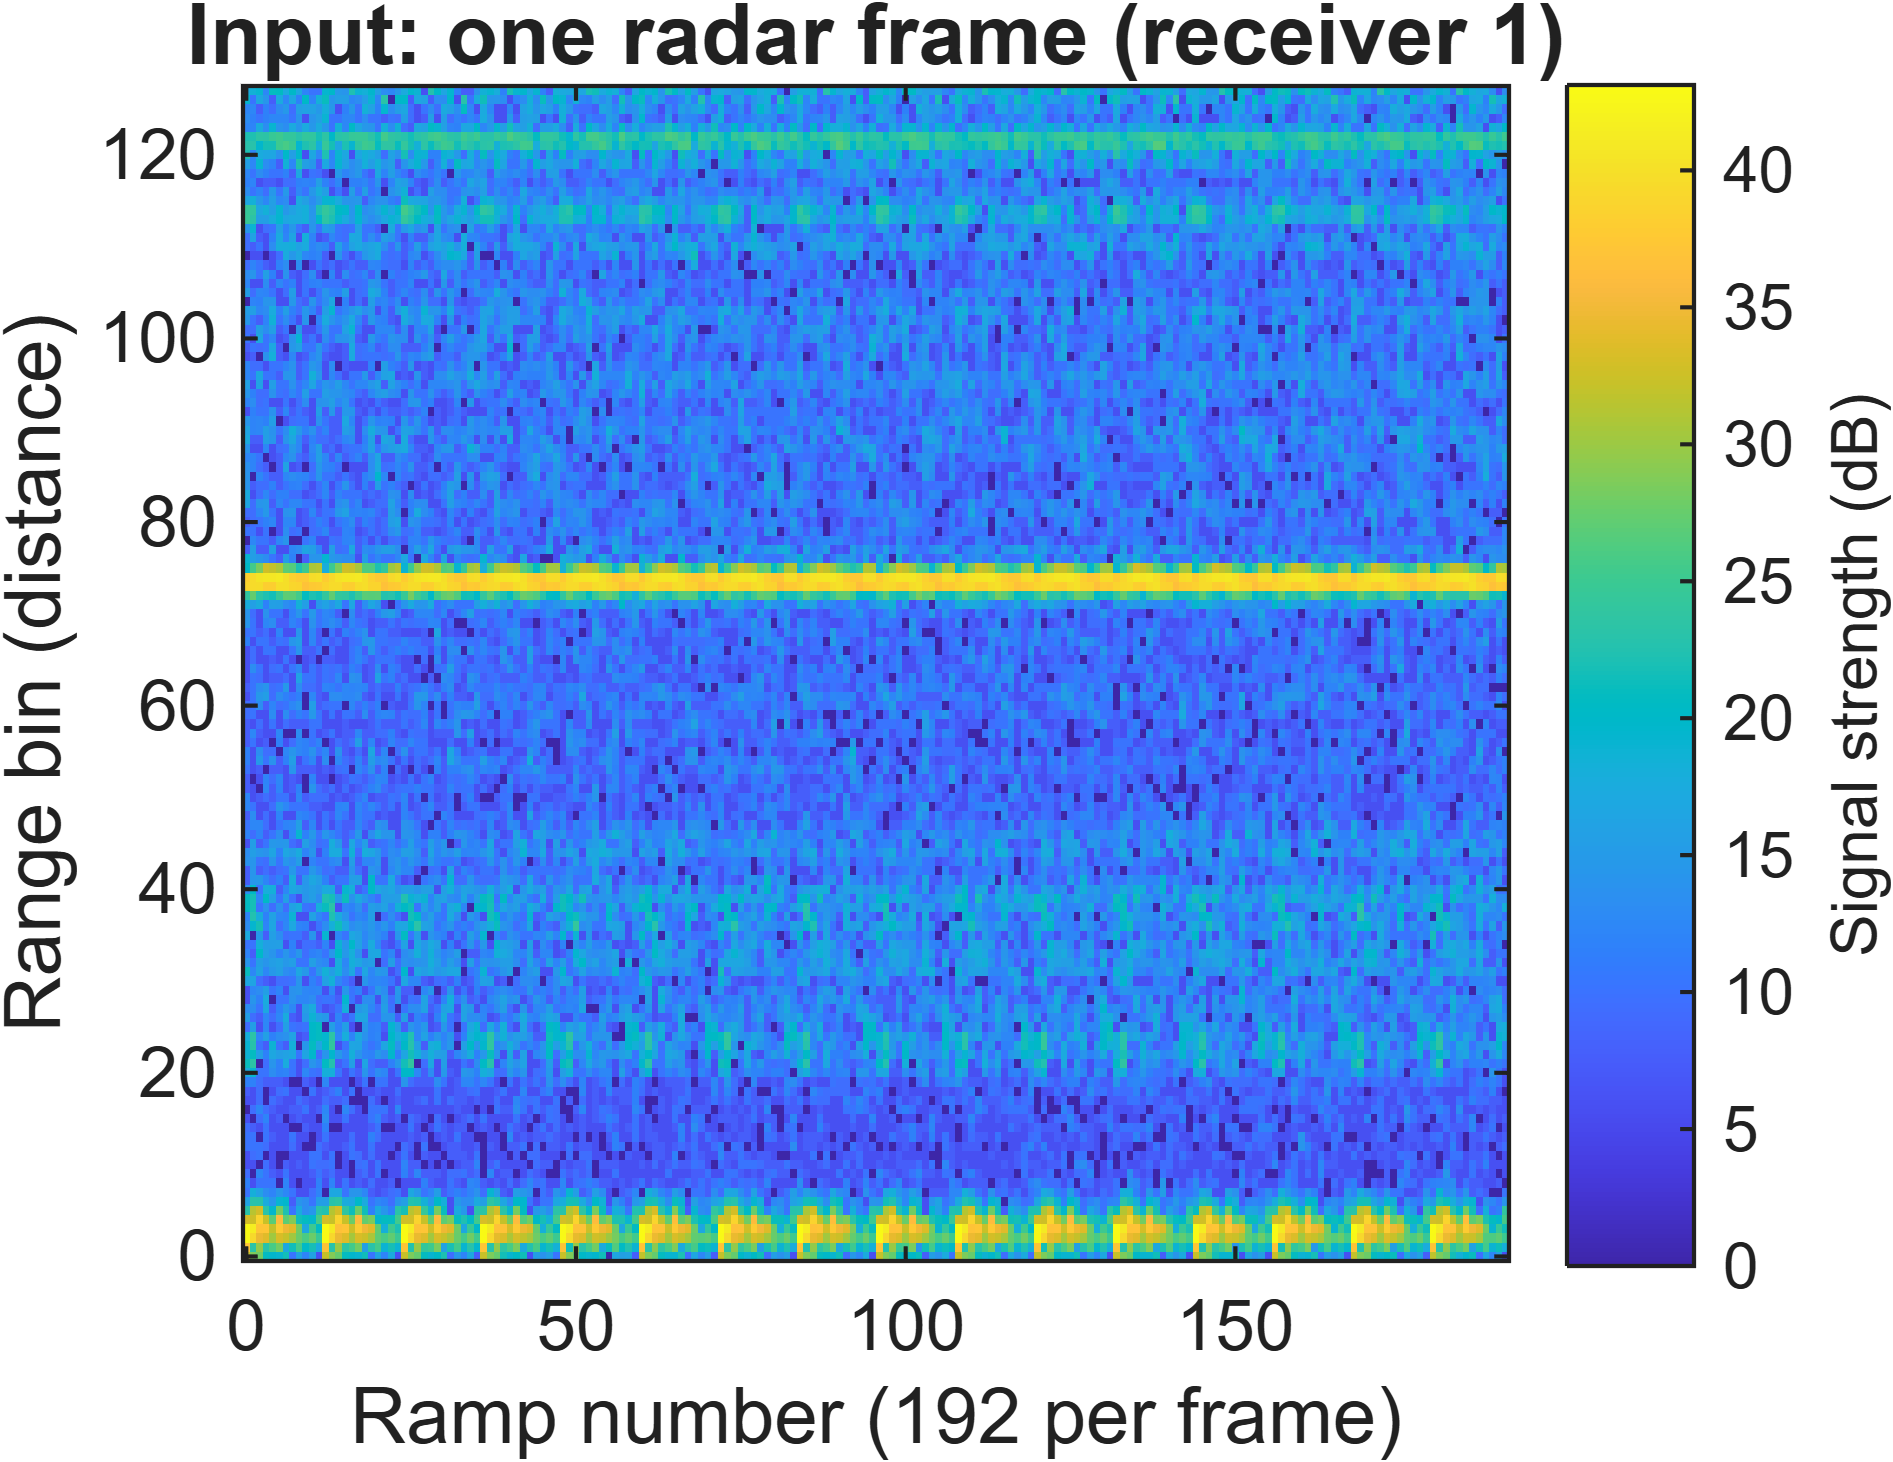
\includegraphics[width=0.6\textwidth]{fig_input.png}
\caption[One input frame]{One input frame as the compressor receives it:
receiver 1 of ColoRadar frame 0 after the range FFT and FX16 quantisation, 128
range bins by 192 ramps. Strong returns appear as horizontal bands at fixed
range; most of the frame is low-level noise, which is why it compresses.}
\label{fig:input}
\end{figure}

For detection, the reconstructed data goes through a 192-point Doppler FFT
across all ramps in recorded order (the transmitter-interleaved axis of
Section~\ref{sec:tdm}), non-coherent integration over the 16 receive channels,
and a detector whose threshold is the mean of the lowest \SI{75}{\percent} of
magnitudes plus \SI{15}{\decibel}, with 8-connected local-maximum suppression.
There is no angle FFT. None of this affects a lossless result, which returns
the input exactly; it matters only for the lossy comparison points.

\section{Metrics}
\label{sec:metrics}

\paragraph{Compression ratio.}
\begin{equation}
\mathrm{CR} = \frac{B_{\mathrm{in}}}{B_{\mathrm{out}}},
\qquad
B_{\mathrm{in}} = N_{\mathrm{ramps}} \times N \times N_{\mathrm{RX}} \times 32,
\end{equation}
with $B_{\mathrm{out}}$ the compressed length \emph{including} the padding of
the last 256-bit word. Ratios are computed per frame and reported as the mean
over 50 frames.

\paragraph{Losslessness.} The maximum absolute difference between input and
reconstruction over every real and imaginary component must be zero. There is
no tolerance.

\paragraph{Detection.}
\label{sec:detectionmetrics}
With $D_{\mathrm{ref}}$ the detections of the double-precision reference and
$D_{\mathrm{test}}$ those of the reconstructed data,
\begin{equation}
\mathrm{FN}\% = \frac{|D_{\mathrm{ref}} \setminus D_{\mathrm{test}}|}{|D_{\mathrm{ref}}|},
\qquad
\mathrm{FDR}\% = \frac{|D_{\mathrm{test}} \setminus D_{\mathrm{ref}}|}{|D_{\mathrm{test}}|}.
\end{equation}
The first is the share of targets missed. The second is labelled a false
positive rate in Kiem's thesis, but it normalises by the test detections, so it
is a false discovery rate. Matching is cell by cell with no positional
tolerance, and the \SI{15}{\decibel} threshold is not swept. FX16, DRHE and LPC
reconstruct identical data, so their detection metrics are identical by
construction: for the lossless methods they measure the cost of the FX16 step
alone.

\paragraph{Baselines.} Every predictive result is reported against a
\emph{no-prediction baseline}, the FX16 codes fed straight into the same
entropy coder; a predictor that does not beat it is not helping. The order-0
entropy of Equation~\eqref{eq:entropy}, evaluated on the residuals, separates
what the predictor achieves from what the dictionary wastes.

\paragraph{Timing.} \emph{Time per frame} runs from the start of a frame's DMA
transfer to the last output word written. \emph{Throughput} is input bits per
frame divided by it. \emph{Latency} runs from the last input word read from
memory to the last output word written back, measured by the board firmware
with a hardware timer; this is Kiem's definition, and it measures how long the
compressed data lags the raw data.

\section{The verification ladder}
\label{sec:ladder}

A compressor that is \emph{nearly} lossless is useless, so every design is
taken down five levels, each checked against the one above, so that a
discrepancy localises to one transition (Figure~\ref{fig:ladder}).

\begin{figure}[t]
\centering
\begin{tikzpicture}[font=\small,
  ph/.style={draw=accent,line width=1pt,fill=lightbg,rounded corners=2pt,minimum width=40mm,minimum height=11mm,align=center,font=\scriptsize},
  a/.style={-{Latex[length=1.6mm]},slate}]
\node[ph] (p1) at (0,0)    {\textbf{1. MATLAB}\\double-precision reference};
\node[ph] (p2) at (0,-1.6) {\textbf{2. HLS C-simulation}\\the C++ run as software};
\node[ph] (p3) at (0,-3.2) {\textbf{3. RTL co-simulation}\\the synthesised hardware};
\node[ph] (p4) at (0,-4.8) {\textbf{4. Vivado implementation}\\placed and routed};
\node[ph] (p5) at (0,-6.4) {\textbf{5. KCU116 board}\\the real system};
\draw[a] (p1) -- (p2); \draw[a] (p2) -- (p3); \draw[a] (p3) -- (p4); \draw[a] (p4) -- (p5);
\node[font=\scriptsize,text=slate,anchor=west,align=left] at (2.5,0)
  {all eight methods; exact bit counts,\\detection metrics};
\node[font=\scriptsize,text=slate,anchor=west,align=left] at (2.5,-1.6)
  {does the C++ reproduce MATLAB \emph{bit for bit}?\\does the decoder recover every sample?};
\node[font=\scriptsize,text=slate,anchor=west,align=left] at (2.5,-3.2)
  {does synthesis preserve it?\\cycle-accurate latency};
\node[font=\scriptsize,text=slate,anchor=west,align=left] at (2.5,-4.8)
  {routed resources and timing\\for the whole system};
\node[font=\scriptsize,text=slate,anchor=west,align=left] at (2.5,-6.4)
  {output byte-identical to C-simulation?\\measured time, throughput, latency};
\end{tikzpicture}
\caption[The verification ladder]{The verification ladder. Each level is checked
against the one above it, so a mismatch localises to a single transition rather
than to ``somewhere in the design''.}
\label{fig:ladder}
\end{figure}

\textbf{MATLAB} models the chain in double precision and gives the exact bits
each algorithm should produce. \textbf{HLS C-simulation} compiles the hardware
C++ as software, on stimulus exported from MATLAB as \texttt{int16}, and checks
over all 50 frames that it produces exactly MATLAB's bit counts and that the
decompressor recovers every sample. \textbf{RTL co-simulation} runs the same
testbench on the generated Verilog for one frame, to check that synthesis
preserved behaviour and to count cycles. \textbf{Vivado implementation} places
and routes the complete board system and gives real resources and timing.
\textbf{The board} streams all 50 frames through the cores and compares the
output byte for byte with the C-simulation.

\section{Edge-case testing}
\label{sec:edgecases}

Real data exercises the typical case well and the extreme case not at all. The
ColoRadar residuals span roughly $[-514, +416]$, which is entirely inside
category 10 of a 16-category code. Everything above that is never exercised by real data.

An eight-case synthetic testbench was therefore built
(Table~\ref{tab:edgecases}), generating its stimulus internally so that it runs
identically in C-simulation and co-simulation.

\begin{table}[t]
\centering
\caption[Synthetic edge cases]{The synthetic edge-case suite. Each case has its
own allowed reconstruction error --- zero for all but the three that can
produce the value $-32768$ and therefore exercise the saturation described in
Section~\ref{sec:robust}. Uniformly random \texttt{int16} input produces a
residual of $-32768$ by chance, so it is one of them.}
\label{tab:edgecases}
\small
\begin{tabular}{@{}llc@{}}
\toprule
Case & What it exercises & Allowed $\mathrm{MaxDiff}$ \\
\midrule
all-zeros        & the $S_4 = 0$ path and the best case & 0 \\
dc-constant      & a perfectly predictable sequence & 0 \\
random-int16     & the worst case: incompressible input & 1 \\
tone-192ramp     & a periodic sequence the AR model should fit & 0 \\
tone-1ramp       & a sequence too short to fit & 0 \\
max-amplitude    & full-scale values, and 128-bit correlations & 0 \\
max-alternating  & $\pm 32767$ alternating: the largest residuals & 1 \\
int16-min        & $-32768$ specifically & 1 \\
\bottomrule
\end{tabular}
\end{table}

The suite exercises the parts of the design that real data never reaches,
including the two situations handled by the robustness measures of
Section~\ref{sec:robust}, neither of which can arise on ColoRadar data.

\section{An independent implementation}
\label{sec:indep}

As a final check that the compression figures are right --- not merely
consistent between MATLAB and C++, which share a specification and could share
a misunderstanding --- the whole compression chain was written a third time,
independently, in Python and NumPy, from the descriptions in
Chapters~\ref{ch:methods} and~\ref{ch:evaluation} without reusing any code. It
reads raw ColoRadar frames, applies the TDM flattening, DC removal, window,
range FFT and FX16 scaling, runs DRHE and LPC with the same coefficient
quantisation as the hardware, and counts the bits of the $S_4$, APPEND and
Huffman coder with and without 256-bit padding. With the original dictionary
it reproduces the HLS bit counts of both algorithms exactly on every one of the
50 frames, and with the re-derived dictionaries it reproduces the hardware's
residuals exactly on the frames checked. It is also the
source of the no-prediction baseline, the entropy figures and the LPC
coefficient statistics reported in Chapter~\ref{ch:results}.
Appendix~\ref{app:verify} lists what was checked.

\section{Tools}

All MATLAB work used R2026a with the Signal Processing Toolbox. All hardware
work used AMD Vitis HLS 2026.1 and Vivado 2026.1, targeting the
\texttt{xcku5p-ffvb676-2-e} device of the KCU116 at a \SI{100}{\mega\hertz}
clock, with XSIM for co-simulation and Vitis for the MicroBlaze firmware. The
board is controlled from a host PC over JTAG with \texttt{xsdb} scripts, and
results are checked with Python. Appendix~\ref{app:repro} lists the source
files and build commands.
